\documentclass[tikz,border=3mm, convert={outfile=compiler.png}]{standalone}
\usepackage{tikz}
\usetikzlibrary{shapes.geometric,positioning}
\begin{document}

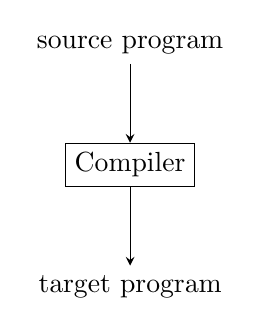
\begin{tikzpicture}[>=stealth]
  % Draw the labelled box. ``compiler'' is its label, and how
  % it is referred to within this TikZ picture. Its displayed
  % text is ``Compiler''. I.e. generically we'd write
  %
  % \node [draw] (nodelabel) {some text};
  %
  \node [draw] (compiler) {Compiler};

  % Create an input node, with the text ``source program'' 
  % which is above the box named ``compiler'', see above.
  \node [above=of compiler] (input) {source program};

  % Create an output node, with the text ``target program'' 
  % which is below the box named ``compiler'', see above.
  \node [below=of compiler] (output) {target program};

  % Draw an arrow _from_ the input node, to the compiler node.
  \draw [->] (input) -- (compiler);

  % Draw an array _from_ the compiler node to the output node.
  \draw [->] (compiler) -- (output);
\end{tikzpicture}
\end{document}
